%
% Angepasste FOM Seminarvorlage
%
\documentclass[12pt,a4paper,listof=totoc,bibliography=totoc]{scrartcl}

\usepackage[english]{babel}			% englische Namen/Umlaute
\usepackage[utf8]{inputenc}	    	% Zeichensatzkodierung
\usepackage{fancyhdr}
\usepackage{graphicx}               % Einbinden von Bildern
\usepackage[hidelinks]{hyperref}	% Klickbare Verweise und \autoref{label}
\usepackage[intoc]{nomencl}
\usepackage{setspace}
\usepackage{parskip}
\usepackage{caption}
\usepackage{float}
\usepackage{geometry}
 \geometry{a4paper, left=40mm, right=20mm, top=40mm, bottom=20mm}
\renewcommand{\familydefault}{\sfdefault}

% Bildueberschrift oben und rechtsbuendig
\captionsetup[figure]{labelfont=bf, textfont=bf}
\captionsetup{justification=raggedright,singlelinecheck=false}

%
%	Hier werden Titel, Bearbeiter und das Datum eingetragen
%
\newcommand\svthema{Supporting Governance and Security in Enterprise IT through Templating and Infrastructure-as-Code}
\newcommand\svperson{Christian Frank (\#473088)}
\newcommand\svdatum{\today}
\newcommand\lvname{Wirtschaftsinformatik: IT-Management}
\newcommand\lvtyp{SS 2020}
\newcommand\lvinst{FOM - Hochschule für Oekonomie \& Management}
\newcommand\lvbetr{Dipl. Ing. (FH) Jan Quatram M.A.}

\hypersetup{ % Thema und Author in die Meta-Daten der PDF
  pdftitle={\svthema}, 
  pdfauthor={Christian Frank},
  pdfsubject={Exploring Rancher and Terraform to support Security and enforce Governance in Enterprise IT},
  pdfkeywords={Rancher, Terraform, Kubernetes, Security, Governance}
}

\begin{document}

% Titel
\title{ \huge\textbf{\svthema} }
\author{ {\svperson} \\ \svdatum }
\date{ \normalsize \centering 
\includegraphics[width=0.3\textwidth]{FOM}\\ {\lvname} \\ {\lvbetr} \\ {\lvinst} \\ {\lvtyp} }

% Seitennummer oben
\pagestyle{fancy}
\fancyhf{}
\fancyhf[ch]{\thepage}
\renewcommand\headrulewidth{0pt}

\maketitle
\thispagestyle{empty} % laesst die Seitennummer auf der Titelseite verschwinden
\pagenumbering{Roman}

\begin{abstract}
In this paper, we'll first have a look at Infrastructure-as-Code frameworks. After introducing the most popular tool, Terraform, we'll look at challenges for Enterprises to manage security and for container environments.
For a possible solution, we'll look at combining Terraform with Rancher from Rancher Inc., a solution that offers exciting features to manage multiple clusters. In closing, we'll look at future developments in security and governance.

\end{abstract}

\vfill
\begin{figure}[h]
    \centering
    
\includegraphics[]{CC-BY}
\end{figure}

This work is licensed under the Creative Commons Attribution 4.0 International License. To view a copy of this license, visit http://creativecommons.org/licenses/by/4.0/ or send a letter to Creative Commons, PO Box 1866, Mountain View, CA 94042, USA.

\cleardoublepage

\tableofcontents			% Inhaltsverzeichnis
\cleardoublepage

\listoffigures				% Abbildungsverzeichnis
\cleardoublepage

%
% Abkuerzungsverzeichnis
%
\makenomenclature
\renewcommand{\nomname}{List of Abbreviations}

\nomenclature{\textbf{ARM}}{Azure Resource Manager}
\nomenclature{\textbf{CI/CD}}{Continuous Integration / Continuous Deployment}
\nomenclature{\textbf{CIS}}{Center for Internet Security}
\nomenclature{\textbf{CLI}}{Command-Line Interface}
\nomenclature{\textbf{CNCF}}{Cloud Native Computing Foundation}
\nomenclature{\textbf{GRC}}{Governance, risk and compliance}
\nomenclature{\textbf{IaaS}}{Infrastructure as a Service}
\nomenclature{\textbf{IaC}}{Infrastructure as Code}
\nomenclature{\textbf{IEC}}{International Electrotechnical Commission}
\nomenclature{\textbf{ISO}}{International Organization for Standardization}
\nomenclature{\textbf{IT}}{Information Technology}
\nomenclature{\textbf{K3s}}{Kubernetes on the edge}
\nomenclature{\textbf{K8s}}{Kubernetes}
\nomenclature{\textbf{NIST}}{National Institute of Standards and Technology}
\nomenclature{\textbf{PaaS}}{Platform as a Service}
\nomenclature{\textbf{PSP}}{Pod Security Policy}
\nomenclature{\textbf{RBAC}}{Role-Based Access Control}
\nomenclature{\textbf{REST}}{Representational State Transfer}
\nomenclature{\textbf{SaaS}}{Software as a Service}
\nomenclature{\textbf{SOX}}{Sarbanes–Oxley Act}
\nomenclature{\textbf{YAML}}{YAML Ain't Markup Language}

\printnomenclature[1.5in]          % Abkuerzungsverzeichnis
\cleardoublepage

\pagenumbering{arabic}
\setcounter{page}{5}

%
%	Einfuehrung
%

\pagebreak
\section{Introduction into Governance and Security}

\onehalfspacing

\subsection{Pronouns}

As we're moving towards a more gender-fluid society, it's time to re-think the usage of gendered pronouns in scientific texts. Two well-known professors from UCLA, Abigail C. Saguy and Juliet A. Williams, argue that it makes a lot of sense to use singular they/them instead: "The universal singular they is inclusive of people who identify as male, female or nonbinary."\footnote{\textit{Saguy, A. (2020)}: Why We Should All Use They/Them Pronouns. \cite{pronouns}} Throughout this text, I'll attempt to follow that suggestion and invite my readers to do the same for their own papers, and support gender inclusivity through gender neutral language. Thank you!

\subsection{Governance vs. Compliance}

In IT it is quite common to use the terms governance and compliance interchangeably. We use the term governance to refer to the process of defining and adhering to a set of operational standards for the overall IT organization. If we look at the formal definition of IT governance in ISO/IEC 38500:2015 though, it is much more focused on the business aspect of running IT. IT governance, as defined by ISO/IEC, will have a heavy emphasis on budgetary control, financial performance and investments. Adherence to standards, such as the Sarbanes–Oxley Act, is more seen as part of compliance than of governance.

However, both, governance and compliance, are part of the overall governance, risk and compliance (GRC) practice in an IT organization and have to go hand in hand.

Throughout the remainder of the document I will use the term governance to refer to all three aspects, governance, risk and compliance.

\subsection{Security}

Throughout the last decade, IT operations have seen their primary focus shift from an on-premise, dedicated environment to shared, on-demand infrastructure, to cloud computing.

The National Institute of Standards and Technology (NIST) defines cloud computing as "a model for enabling ubiquitous, convenient, on-demand network access to a shared pool of configurable computing resources (e.g., networks, servers, storage, applications, and services) that can be rapidly provisioned and released with minimal management effort or service provider interaction."\footnote{\textit{Mell, P. (2011)}: The NIST Definition of Cloud Computing. \cite{sp800-145}}

In the early days of cloud computing, virtualization played a key role and drove adoption; a couple of years ago the focus shifted away from virtualization towards containerization. All major Hyperscalers now have container run-time offerings, managed and unmanaged, based on the Kubernetes orchestration framework.

Container run-time environments have their own important security aspects, as outlined by NIST.\footnote{See \textit{Souppaya, M. (2017)}: Application Container Security Guide. \cite{sp800-190}}

For the purpose of this document, we'll concentrate on the aspects of security and governance (regulatory compliance) in container run-time environments.


%
%	Begrifflichkeiten
%

\pagebreak
\section{The need for Governance and Security in container run-time environments}

\onehalfspacing

\subsection{Container Run-Time Environments}

Let's start with the basics. In most of IT, Kubernetes\footnote{See \textit{The Linux Foundation (2020)}: Production-Grade Container Orchestration. \cite{kubernetes}} has emerged as the container run-time environment of choice.

Earlier competitors, such as Docker Swarm or Mesos DC/OS, have all but vanished. After Mirantis acquired Swarm from Docker last year, they announced a two-year end-of-life timeline for support, but they have since announced that they might extend this and possibly invest in new features.

The original platforms that spawned cloud-native computing and application design and gave us the concept of micro-services, Heroku and Cloud Foundry, have also slightly gone out of favor, or, in the case of Cloud Foundry, moved to a Kubernetes-based run-time. Salesforce.com acquired Heroku in 2010; an independent foundation, led by VMware, owns Cloud Foundry with SUSE playing a very active part.

In a previous paper, I have covered Kubernetes in more detail\footnote{See \textit{Frank, C. (2020)}: Multi-Cluster Management fuer Containerumgebungen .\cite{previousPaper}}, in this paper I will only cover the necessary basics.

\subsection{Kubernetes Architecture}

A Kubernetes container run-time environment, or cluster, in general, will consist of one or more logically grouped systems. These systems, most likely virtual machines, will run a supported container run-time, such as Docker (Microsoft / Ubuntu) or Podman (Red Hat).

A single Kubernetes cluster has a Control Plane and an Execution Plane. Usually, there are three nodes in the control plane and one or more nodes in the execution plane. For the control plane, you should choose an odd number of nodes because the underlying etcd database is a distributed system and needs to reach quorum on startup. The number of worker nodes in the execution plane only depends on the needs of your application.

The Kubernetes control plane takes care of orchestrating the application deployments and maintains their state; on the other hand, the worker nodes execute the actual application containers as defined and scheduled by the control plane. Worker nodes can be organized into one or more node pools to separate hardware features or reliability aspects.

In addition to providing compute nodes, Kubernetes includes overlay networks to allow communication between the cluster nodes, and ingress controllers for inbound network access to the running applications. Persistent storage, even though it's an anathema to stateless, cloud-native computing, is provided through persistent volumes and storage classes and linked to the underlying cloud provider.

All administrative access to a given Kubernetes cluster is via the master nodes and its Kubernetes API endpoint.

\subsection{Kubernetes Security}

Installing the first Kubernetes cluster is no longer a big task, especially on the three big public cloud providers, which all offer managed Kubernetes clusters with easy, one-click installations.

However, designing the platform landscape requires some architectural knowledge and should be planned well in advance.

One of the crucial components of security when running containers in production, according to NIST, is the separation between applications and systems. Put careful consideration during design into the number and type of Kubernetes clusters deployed.\footnote{See \textit{Weibel, D. (2020)}: Architecting Kubernetes clusters. \cite{howMany}}

Kubernetes itself, at the time of writing, does not provide for hard tenancy. Breakouts and cross-talk remain a possibility. To entirely separate applications on all layers (compute, network, and storage), using multiple clusters is a good option. Many enterprises might thus end up with more than one Kubernetes cluster, sometimes with many more. This will, of course, have a significant effect on operations.

With the increase in popularity, Kubernetes also brings other new security challenges that should be considered when designing the IT environment.\footnote{See \textit{Weizmann, Y. (2020)}: Threat matrix for Kubernetes. \cite{threatMatrix}}

We're observing a trend in Enterprise IT to move from traditional perimeter-based network security to more modern zero- or low-trust networks with identity-based security and temporary infrastructure. Having multiple, short-lived Kubernetes cluster is thus an entirely likely scenario going forward.

\subsection{Rancher Overview}

To easily manage a set of Kubernetes clusters, we can turn to Rancher.

What is Rancher? According to the Rancher Labs website, it is "[...] a complete software stack for teams adopting containers. It addresses the operational and security challenges of managing multiple Kubernetes clusters, while providing DevOps teams with integrated tools for running containerized workloads"\footnote{\textit{Rancher Labs (2019)}: Run Kubernetes Everywhere. \cite{rancher}}

Rancher provides a management platform to centrally manage multiple Kubernetes clusters in Enterprise IT, all from a choice of two user-friendly GUIs. Rancher also offers integration tools for application development and robust enterprise-grade features for security and governance. For operations, Rancher provides integrated solutions for logging, monitoring, and auditing, together with many other features, such as CIS scans or a built-in service mesh.

The classic Rancher GUI looks like this:

\begin{figure}[H]
\centering
\caption {Rancher Overview}
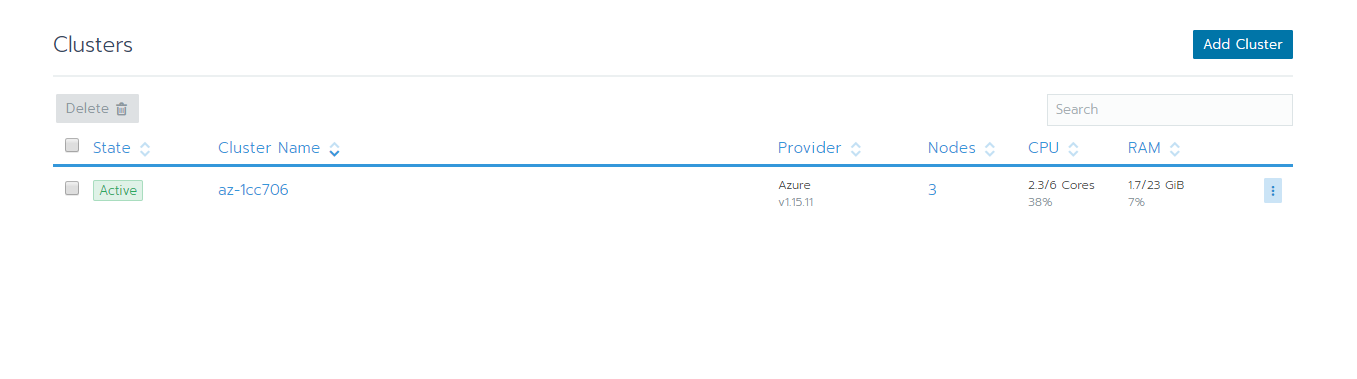
\includegraphics[width=\linewidth]{images/cluster-overview.png}
\label{fig:rancherOverview}
\end{figure}

\subsection{Rancher Architecture}

Rancher is, similar to Kubernetes, itself a containerized application and can be installed from a single image to a single Docker host. Such a single-node installation is ideal for test-beds or local Rancher installations on a laptop, for example. A single node installation does not provide any redundancy in case of failure.

For production installations, Rancher can be installed on a separate Kubernetes cluster, using Kubernetes' redundancy mechanisms for high-availability and resiliency. It could either be co-hosted on an existing cluster or better, on a small, separate infrastructure cluster. Installation on a separate cluster is the recommended choice. It is good practice in IT to keep administrative tools on separate infrastructure from the administered infrastructure, and thus the installation on a different cluster is the most widespread.

In addition to the GUI, the Rancher server also provides a central Kubernetes API endpoint, which prevents unauthorized access and sits as an intermediary between the users and the actual Kubernetes clusters.

You can find more details on the Rancher architecture in Rancher's technical architecture document.\footnote{See \textit{Rancher Labs (2020)}: Rancher Technical Architecture. \cite{technicalArchitecture}}

The open-source Kubernetes run-time threat detection engine Falco works very well with Rancher.\footnote{See \textit{Shankar, P. (2020)}: Runtime Security in Rancher with Falco. \cite{falcoPsp}}

I've covered the aspect of cluster and workload segmentation in more detail in my previous FOM paper on multi-cluster management in Enterprise IT. I've also explained in that paper as to why I view the combination of Kubernetes and Rancher as a very beneficial one, especially for Enterprise IT.\footnote{See \textit{Frank, C. (2020)}: Multi-Cluster Management fuer Containerumgebungen .\cite{previousPaper}} 


%
%	Theorieteil
%

\pagebreak
\section{Governance and Security in the Enterprise}

\onehalfspacing

\subsection{Key requirements for Kubernetes cluster in Enterprise IT}

Installing the first Kubernetes cluster is not a big task anymore, especially on the three big public cloud providers, which all offer managed Kubernetes clusters with easy, one-click installations.

Designing the platform landscape, however, does need some architectural knowledge and should be planned well in advance.

Once the transition to cloud-native application development begins, the DevOps teams are in place, and application deployment with containers is introduced to IT production, Day Two operations and security become the primary concerns.

One of the crucial components of security when running containers in production, according to NIST, is the separation in between applications and systems.\footnote{See \textit{Souppaya, M. (2017)}: Application Container Security Guide. \cite{sp800-190}}

\begin{figure}[h]
\centering
\caption {Cluster Separation}
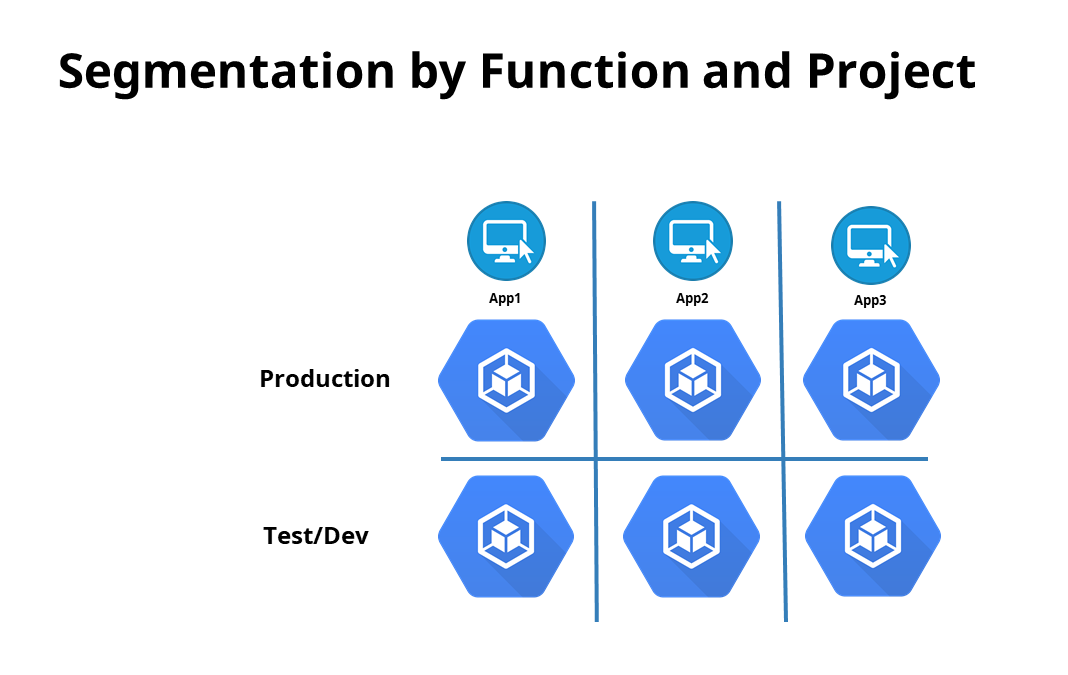
\includegraphics[width=\linewidth]{images/separation}
\label{fig:clusterSeparation}
\end{figure}

Segmentation of applications could be performed along the lines of function (Production, Development/Test), or between applications, or both. In single-cluster environments, separation could be achieved through networking or otherwise through the introduction of multiple clusters. 

A key consideration when implementing separation is the so-called "Blast Radius", a term borrowed from the military, which depicts the amount of damage an explosive would cause. IT uses it to assess the damage a breach, data loss, or failure of a given IT system would cause to the whole operation, in technical and financial terms.

Defining application and data security classes is part of the preparation process when introducing containers to production, and would exceed the scope of this paper.

Kubernetes itself, at the time of writing, does not provide for hard tenancy. To entirely separate applications on all layers (compute, network, and storage), the use of multiple clusters is a good option. Many enterprises might thus end up with more than one Kubernetes cluster, sometimes with many more, which will, in turn, have a significant effect on operations.

We're observing a trend in Enterprise IT to move from traditional perimeter-based network security to more modern zero- or low-trust networks with identity-based security and temporary infrastructure. Having multiple, short-lived Kubernetes cluster is a likely scenario going forward.

\subsection{The principle of least privilege}

The second crucial component of security is user authentication and authorization; especially with the shift towards identity-based security, Enterprise IT needs to establish a trusted identity provider and link it to its container platform.

Many Enterprise IT already have some form of central user authentication through Microsoft Active Directory or any other Single-Sign-On provider. Kubernetes has built-in Role-Based Access Control and can restrict access to its resources based on the roles bound to a specific user or object.

Defining Roles and Responsibilities is part of the Role Engineering process during the introduction of containers, and would exceed the scope of this paper. It is, however, necessary in RBAC to fully embrace the principle of least privilege - only ever grant the minimum access rights required to fulfill the job without jeopardizing efficiency. 

A comprehensive reference for RBAC is in David F. Ferraiolo's book of the same name, Role-Based Access Control\cite{rbac}.

\subsection{Organizational considerations}

The third crucial component of security is departmental organization - NIST recommends that an organization changes its operational culture and technical processes to embrace and support agile application development fully.

Agile software development requires an agile organizational structure and self-organized teams to support the agile mantra “You build it, you run it” (Werner Vogels).\footnote{\textit{Orban, S. (2015)}: Enterprise DevOps: Why You Should Run What You Build. \cite{devOps}}

Without such changes, from experience, the likelihood of failing the transformation to container-based, cloud-native application development is quite high.

\subsection{Day Two operations with multiple Kubernetai}

Once all preparations have been completed, the organizational structure is about to change, and multiple clusters are installed, there are a lot of configuration items and actions that need to be synchronized across all clusters.

Central user authentication and authorization is critical. Authentication can be performed through an identity provider, but roles and responsibilities need to be defined for each cluster, and users need to be assigned the roles for authorization. There's only one hierarchy level on Kubernetes; roles can be bound to user objects and become active in one or more namespaces.

Kubernetes provides two types of security policies, one for pod security and one for network security. Pod security policies, as the name implies, govern security-relevant aspects of pod specification,\footnote{See \textit{The Linux Foundation (2019)}: Pod Security Policies. \cite{podSecurity}} whereas network policies govern the allowed communication between groups of pods and the outside world.\footnote{See \textit{The Linux Foundation (2019)}: Network Policies. \cite{netSecurity}}

As time goes on, supporting applications will need to be updated, and Kubernetes itself might need to be updated unless a public cloud provider manages Kubernetes.

To effectively control a Kubernetes cluster and aid in troubleshooting, logging and monitoring should be configured and enabled.

Kubernetes stores its configuration and metadata information in a distributed database. This information state needs to be regularly backed up, and in case of issues, be restored.

To provide for data persistence, volumes and shared file systems need to be created for various Kubernetes clusters.

For software development and automatic deployment, it makes sense to connect the development pipeline(s) to the respective clusters, have a central image registry and establish central governance for deployment workflows.

For micro-service observability, distributed tracing and network control, a service mesh could be installed - a quite popular choice would be Istio.\footnote{See \textit{Istio Authors (2019)}: Istio - Connect, secure, control, and observe services. \cite{istio}}

All of the tasks above can be performed against individual clusters with native Kubernetes tools, but once there are a couple of clusters to manage, this will get tedious and quite difficult to synchronize.

It will even get more complicated once IaC enters the picture, and Kubernetes clusters are starting to become ephemeral with the run-time environment recreated fresh with each new application deployment, entirely relying on automation to implement governance and policies.

\subsection{Possible solutions}

To address all these issues, CNCF is working on Kubernetes federation and multi-cluster controlling, but the development still in its infancy and not production-ready yet.\footnote{See \textit{sig-multicluster (2019)}: Kubernetes Cluster Federation. \cite{kubeFed}}

The three big cloud providers also provide solutions to manage multiple clusters: Google Cloud has Anthos,\footnote{See \textit{Google (2019)}: Anthos - Bringing the cloud to you. \cite{googleAnthos}} Microsoft Azure has Azure Arc in Preview,\footnote{See \textit{Microsoft (2019)}: Bring Azure services and management to any infrastructure. \cite{azureArc}} and AWS is working on AWS Outposts.\footnote{See \textit{AWS (2019)}: AWS Outposts. \cite{awsOutposts}}

A popular open-source solution for this problem is Rancher from Rancher Labs. In the next chapter, we'll have a look at whether Rancher could provide a solution to Kubernetes multi-cluster management and how it would address the issues outlined above.


%
%	Praxisbezug
%

\pagebreak
\section{CIS Scans}

\onehalfspacing

\subsection{Rancher hardening}

Text.\footnote{See \textit{Rancher Labs (2019)}: Hardening Guide. \cite{hardeningGuide}}

\subsection{CIS Scan GUI}

Text. 

\begin{figure}[H]
\centering
\caption {CIS Scan GUI}
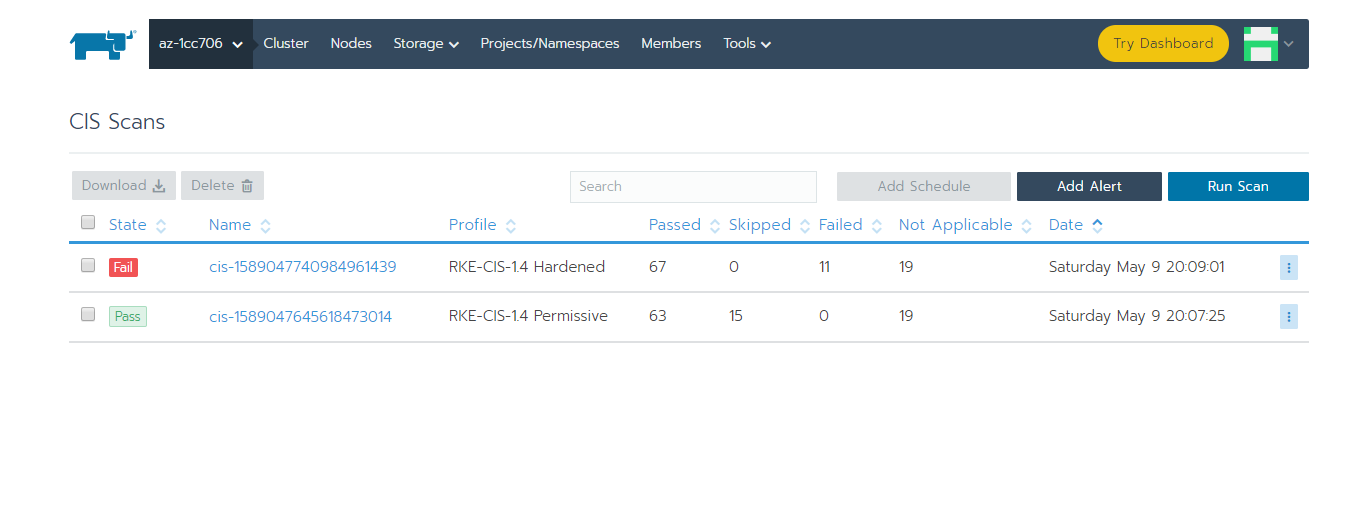
\includegraphics[width=\linewidth]{images/cis-scan-overview.png}
\label{fig:cisScanOverview}
\end{figure}

\subsection{CIS Scan Hardened}

Text. 

\begin{figure}[H]
\centering
\caption {CIS Scan Hardened}
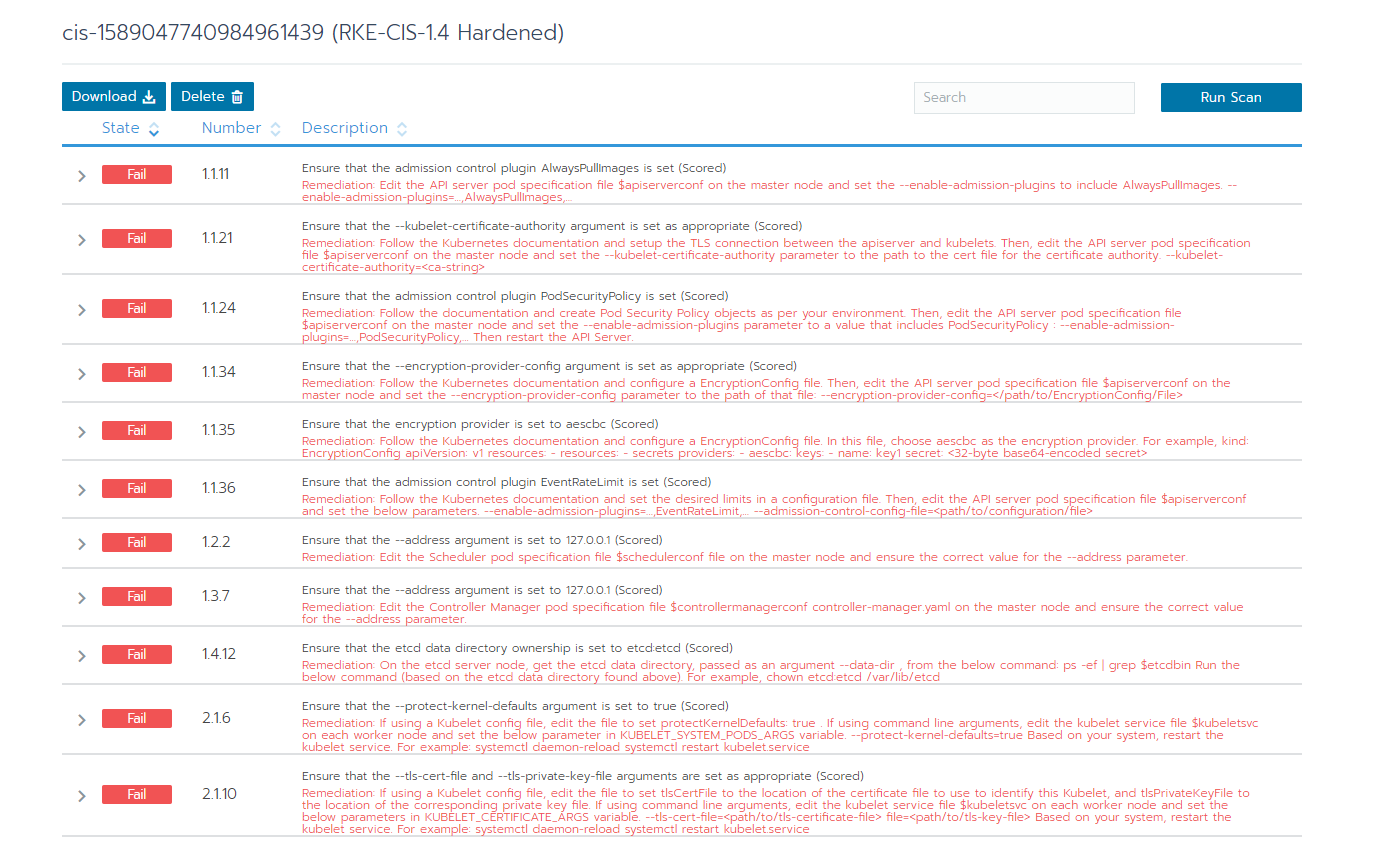
\includegraphics[width=\linewidth]{images/cis-scan-detail.png}
\label{fig:cisScanDetails}
\end{figure}

\subsection{Remediation}

Text.\footnote{See \textit{Rancher Labs (2020)}: Changelog. \cite{ChangeLog}}

Text.\footnote{See \textit{Price, J. (2020)}: Kubernetes - Pod Security Policies. \cite{examplePsp}}

Text.\footnote{See \textit{Iradier, A. (2020)}: Enhancing Kubernetes Security with Pod Security Policies. \cite{detailPsp}}

Text.\footnote{See \textit{Shankar, P. (2020)}: Runtime Security in Rancher with Falco. \cite{falcoPsp}}


%
%	Fazit
%

\pagebreak
\section{Summary and recommendations}

\onehalfspacing

Infrastructure-as-Code is the perfect tool to enforce regulatory compliance and security hardening uniformly across all deployed Kubernetes clusters.

Terraform provides the declarative definition for the infrastructure and Rancher, through templates and access control, the necessary controls for the installation and configuration of Kubernetes itself.

The Center of Internet Security offers benchmarks, to test Kubernetes cluster against. Rancher has CIS Scans integrated and offers the ability to mitigate the findings.

We were able to show that the combination of Terraform together with Rancher templates provides an ideal solution for Enterprise IT to provision a secure and compliant container run-time environment and manage the infrastructure life cycle. By having all infrastructure well defined and under revision control, and all infrastructure deployments automated, GRC controls can be applied easilly. 

There are alternatives to this combination. Platform-native solutions for the major hyperscale platforms do exist, for example ARM templates on Microsoft Azure or Cloud Formation on Amazon Web Services. Also, the leading on-premise virtualization platforms, VMware and Hyper-V, each have a native orchestration solution as well.

Rancher and Terraform, however, are an open-source and provider-independent
option and thus the recommended choice; both tools have been around for a couple of years and amassed a large and largely loyal user base.

There are other open-source tools, such as the very recently released CDK8S by Amazon Web Services, but in my opinion Rancher and Terraform remain the most comprehensive option and are ideally suited for cloud computing.

Infrastructure automation is by no means a new invention. Procedural tools like Ansible, Chef or Operations Orchestration have been around for decades.

New developments in the area of serverless computing threaten compute infrastructure as a distinct category itself and might obliterate the need for secure and compliant orchestration tools, though.

Regardless of future developments, governance, risk management and regulatory compliance will remain a key topic in Enterprise IT.

You can find all example plan files on my  \href{https://github.com/chfrank-cgn/Rancher/tree/master/az-cluster-1}{GitHub}.

Happy Ranching!


% Literaturverzeichnis
\cleardoublepage
\raggedright
\bibliographystyle{IEEEtranS}	% ieeetran verwenden, damit auch URLs angezeigt werden
\bibliography{seminar-lit}

%
%	Ehrenwoertliche Erklaerung
%

\pagebreak

\pagenumbering{gobble} % Keine Seitenzahlen mehr
\onehalfspacing

%-----------------------------------
% Ehrenwoertliche Erklärung
%-----------------------------------
\section*{Declaration in lieu of oath}

\par\medskip

I, with this, declare that I produced the submitted paper with no assistance from any other party and without the use of any unauthorized aids and, in particular, that I have marked as quotations all passages which are reproduced verbatim or near-verbatim from publications. Also, I declare that the submitted print version of this thesis is identical to its digital version. Further, I say that this thesis has never been introduced before to any examination board in either its present form or in any other similar version. I herewith agree that this thesis may be published. I herewith consent that this thesis may be uploaded to the server of external contractors to submit it to the contractors’ plagiarism detection systems. Uploading this thesis to send it to plagiarism detection systems is not a form of publication.

\par\medskip
\par\medskip

\vspace{5cm}

\begin{table}[H]
	\begin{tabular*}{\textwidth}{c @{\extracolsep{\fill}} ccccc}
		Cologne, \the\month/\the\day/\the\year \\
		\rule[0.5ex]{12em}{0.55pt} & \rule[0.5ex]{12em}{0.55pt} \\
		(Location, Date) & (Signature)
	\end{tabular*}
\end{table}


\end{document}
